\part{运动分析}
\markboth{运动分析}{运动分析}

\begin{figure}[!htb]
	\centering
	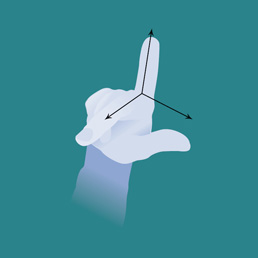
\includegraphics[width=0.4\linewidth]{chap7/7_0_0}
	% 加星号(*)表示不加编号
	\caption*{ \label{fig:7_0_0}}
\end{figure}



\chapter{运动量化} \label{chap:chap7}


并非所有变化都是成长,
正如并非所有运动都是前进。
\begin{flushright}
	——艾伦$\cdot$格拉斯哥
\end{flushright}

\begin{figure}[!htb]
	\centering
	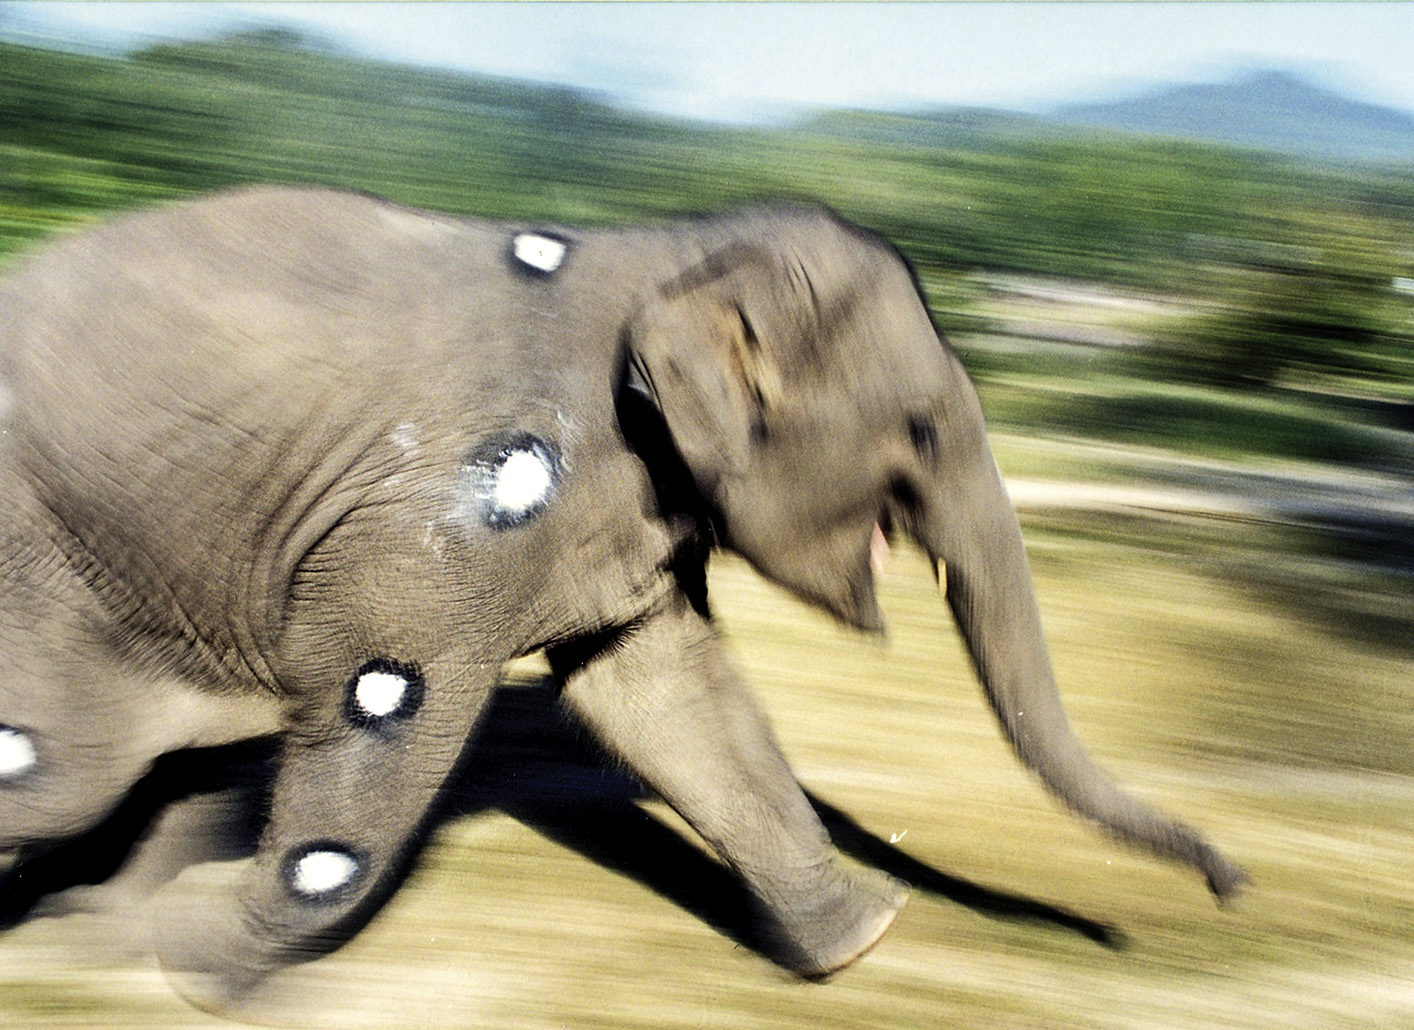
\includegraphics[width=1.0\linewidth]{chap7/7_0}
	% 加星号(*)表示不加编号
	\caption*{ \label{fig:7_0}}
\end{figure}

这是每个足球运动员都害怕的时刻。
落地姿势不对,发出砰的一声。
膝盖剧痛,膝盖再也无法支撑任何重量,瘫倒在地。
队医的检查,以及在这种情况下谁也不想听到的 3 个字母:ACL。
也就是前交叉韧带,膝盖受伤最常见的部位。


或许比最初的疼痛更糟糕的是接下来的伤痛:
外科医生在胫骨和股骨上钻孔,数周佩戴支架,然后是数月的康复治疗。
完成所有这些之后,重返赛场的可能性很大。
但重返赛场并不等同于从此过上幸福的生活。
从前交叉韧带(ACL)受伤中恢复的运动员再次受伤的风险更高,受伤膝盖患关节炎的风险也更高。
比赛结束很久之后,运动员仍将为此付出代价。


如果可以预防 ACL 损伤会怎样?
大多数 ACL 损伤并非由接触引起,许多损伤可以通过注重平衡、正确落地技巧和提升身体姿势意识的训练来预防。
如果针对风险最高的运动员进行训练,效果会更加显著。
测量运动员的动作可以确定他们是否有 ACL 损伤的风险。
他们跳跃落地时膝盖是否对齐(好)或错位(坏)?
他们落地时膝盖是否弯曲以吸收冲击能量(好)或膝盖是否伸展(坏)?


在高水平的体育竞赛中,细节至关重要,没有什么可以替代量化的表现指标。
在科学研究中也是如此。
著名数学物理学家开尔文勋爵(Lord Kelvin)以他的名字命名了绝对温度的单位,他对量化有如下看法\cite{thomson1894popular}:



我经常说,当你可以衡量你所说的内容,并用数字表达出来时,你就对它有所了解;
但是当你无法衡量它,无法用数字表达它时,你的知识就是贫乏和不令人满意的:
这可能是知识的开始,但无论内容是什么,在你的思想中,你都还没有进入科学的阶段。


本章将介绍最常用的运动测量技术,包括测力台和使用摄像机进行运动捕捉。
此外,我们还将介绍确定受试者骨骼姿态的技术,即逆运动学问题。


我们的最终目标是了解产生运动的肌肉力量,但这些力量通常无法直接测量。
因此,我们通过构建骨骼模型并计算与观察到的运动最吻合的关节角度随时间的变化来估算这些肌肉力量(本章)。
然后,我们计算作用于每个关节的力和力矩(第~\ref{chap:chap8}~章),最后解决一个优化问题,该问题反映了身体如何协调数十块肌肉来产生这些力和力矩(第~\ref{chap:chap9}~章)。
显然,我们必须打下坚实的基础才能实现接下来两章更宏伟的目标。
所有后续分析的质量都取决于我们计算关节角度的准确性,这也是本章的主要目标。
但首先,让我们回顾一下历史,看看逆运动学方法是如何发展的。



\section{测量技术}

早期对运动的研究仅限于对整体身体运动的定性观察和测量。
19 世纪摄影技术的进步使摄影变得实用,并为令人兴奋的运动新研究提供了可能。
1872 年,利兰$\cdot$斯坦福(他与妻子简创办了斯坦福大学)试图解决关于马的运动方式的争论。
马在小跑时,会同时用对角线方向的腿向前移动。
斯坦福认为,在小跑的马中有一段时间,它的 4 个蹄子会同时腾空,于是聘请了埃德沃德$\cdot$迈布里奇进行研究。
迈布里奇和工程师约翰$\cdot$艾萨克斯开创了一种拍摄运动中的马的技术,他们使用沿着马的路径放置一系列摄像机,并能够捕捉到小跑马腾空的瞬间。
运动中的马的照片(图~\ref{fig:7_1})彻底改变了生物力学领域,并推动了电影的发展。


\begin{figure}[!htb]
	\centering
	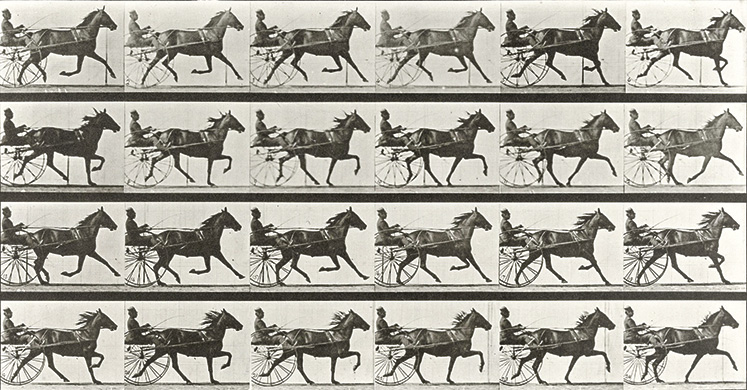
\includegraphics[width=1.0\linewidth]{chap7/7_1}
	\caption{是嘶鸣还是嘶鸣?
		1872年,利兰$\cdot$斯坦福聘请埃德沃德$\cdot$迈布里奇来测试马小跑时四蹄是否同时腾空。
		这组照片中的第四张捕捉到了四蹄同时腾空的瞬间。
		图片由斯坦福大学提供。 \label{fig:7_1}}
\end{figure}


虽然视频分析仍然是生物力学的重要组成部分,但其他用于测量运动的技术也已发展起来。
例如,可以使用荧光透视法获得骨骼的亚毫米级测量值,该技术会连续拍摄X射线图像(图~\ref{fig:7_2})。
遗憾的是,由于暴露于电离辐射(以及视野有限),该技术通常不适用于大规模研究。
此外,还可以通过植入从皮肤突出的骨锚定针并使用光学技术追踪这些针的运动来获得精确的运动学测量值。
正如您所料,这种操作的侵入性使其不适用于大多数研究。


\begin{figure}[!htb]
	\centering
	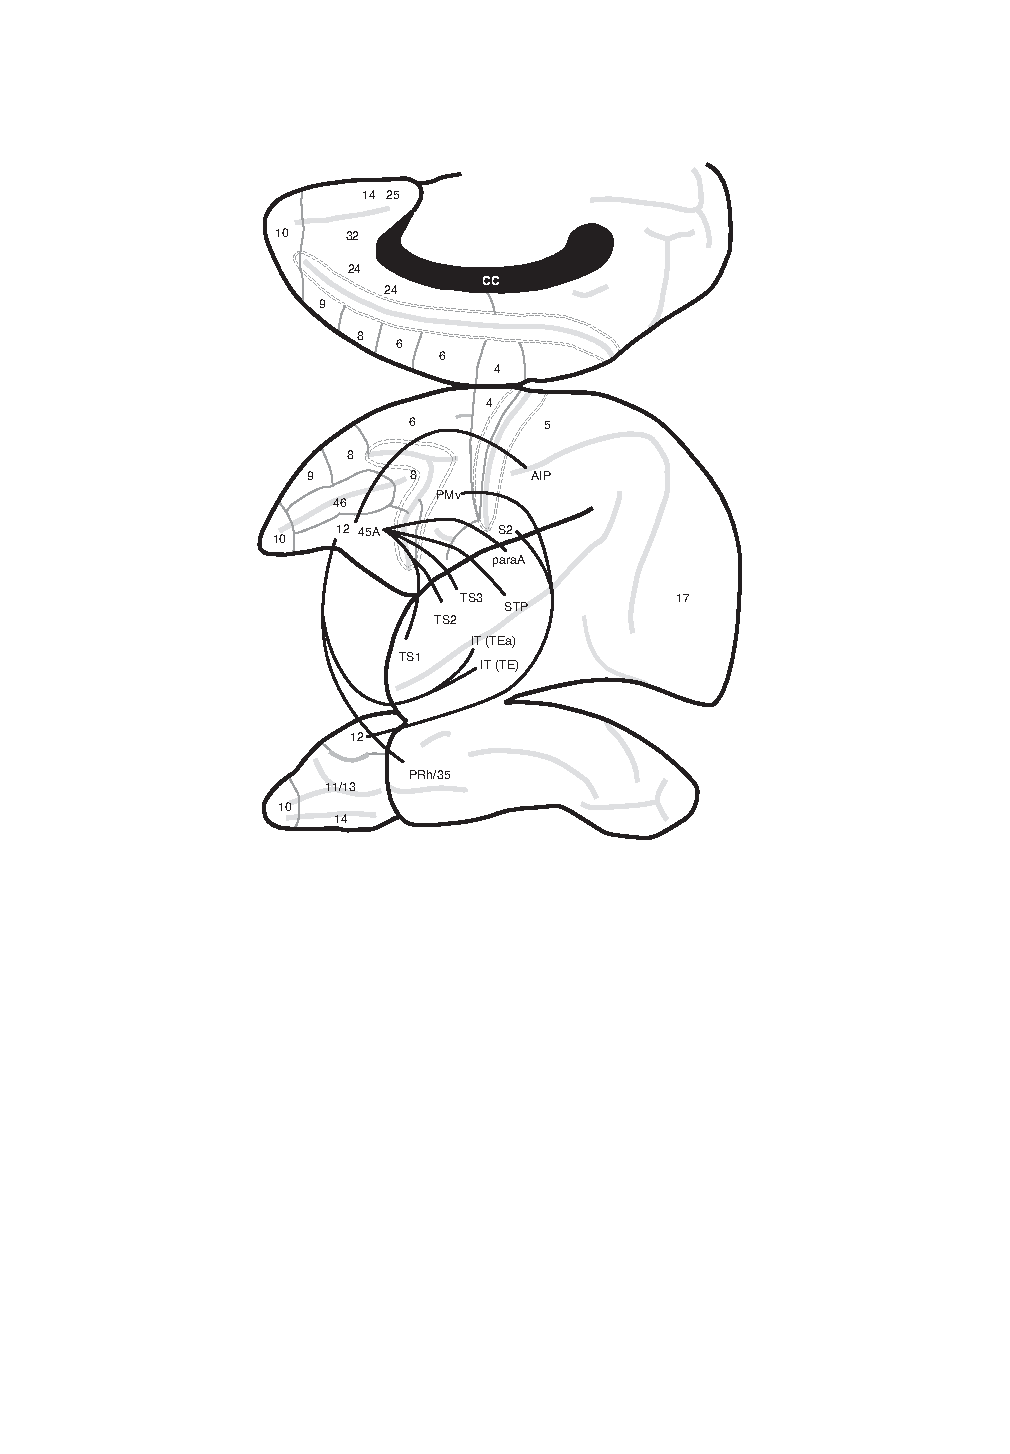
\includegraphics[width=1.0\linewidth]{chap7/7_2}
	\caption{透视图像显示健康肩关节(上排)和全肩关节置换术后(下排)的骨骼运动。
		图片由犹他大学骨科研究实验室提供。。 \label{fig:7_2}}
\end{figure}


惯性测量单元 (IMU) 已成为现有量化运动策略的低成本替代方案,并日益流行。
IMU 通常包含用于测量线性加速度的加速度计、用于测量角速度的陀螺仪以及用于测量相对于磁北方向的航向的磁力计。
在许多研究中,IMU 无需使用摄像头和受控照明条件,这使得人们能够在自然环境中进行生物力学实验,例如在游泳和越野跑等活动中进行实验,并能够长时间捕捉偶发事件或监测健康状况(图~\ref{fig:7_3})。
例如,Helen Bronte-Stewart 使用 IMU 测量受试者在模拟生活环境中行走时每条腿在矢状面上的角速度,而光学运动捕捉在这种环境中是不切实际的。
每个摆动阶段的开始和结束都对应于他们测量的角速度信号的过零点。
该实验装置使他们能够检测帕金森病患者的步态冻结发作(图~\ref{fig:7_4}),这是一种行走突然中断的步态障碍。IMU也已用于测量足球运动员头骨的运动(图~\ref{fig:7_5}),并可用于帮助监测运动员的大脑健康状况。


\begin{figure}[!htb]
	\centering
	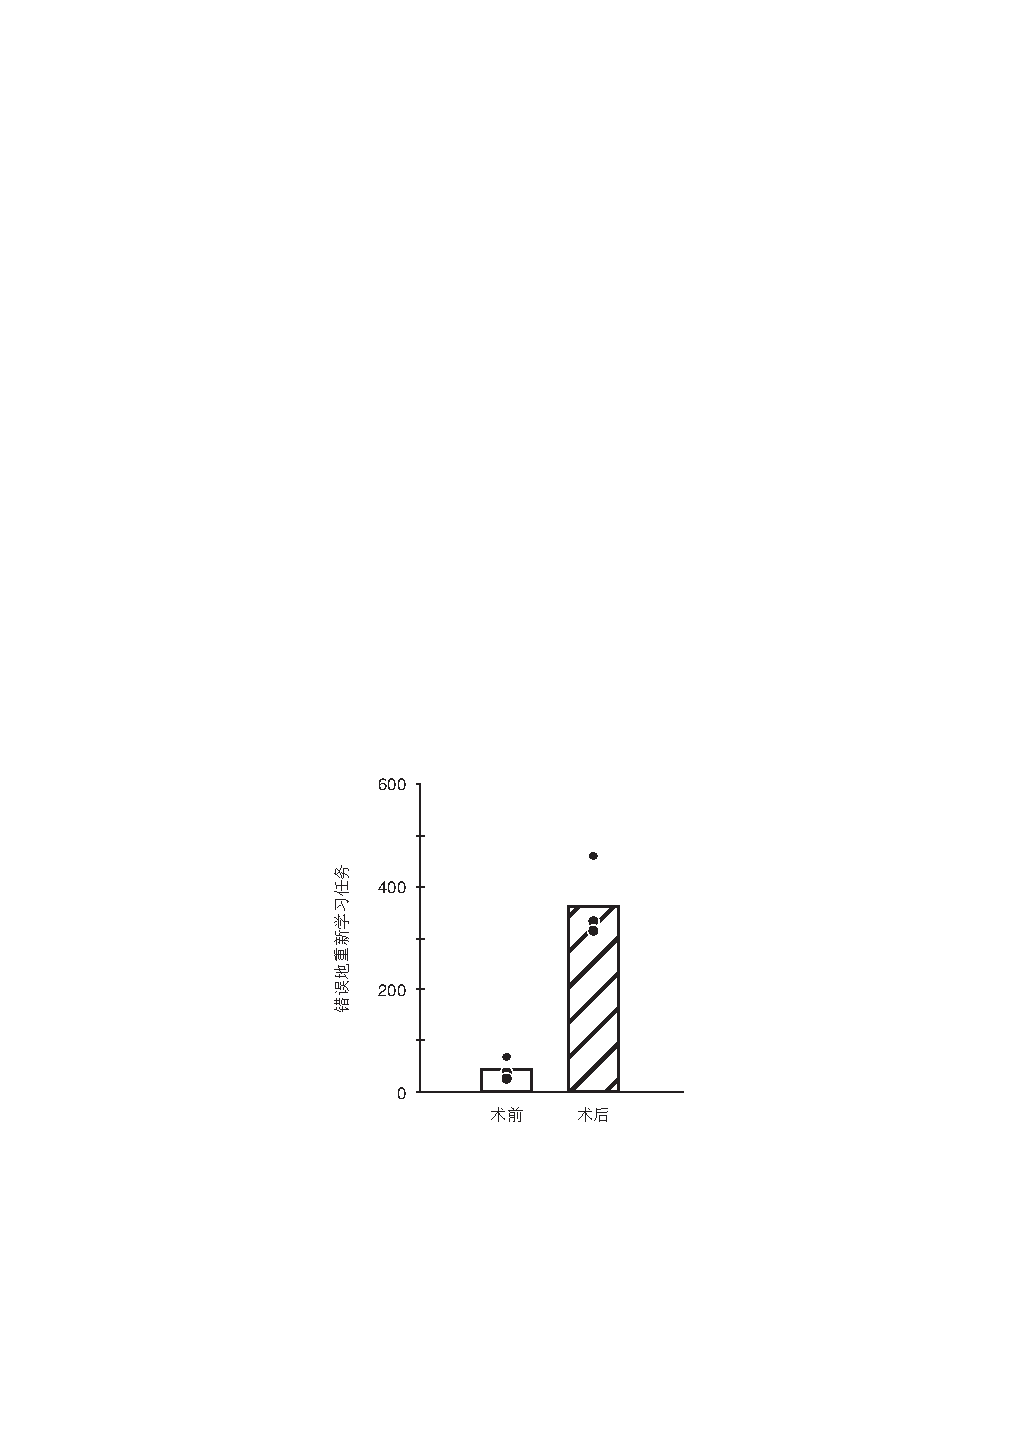
\includegraphics[width=0.6\linewidth]{chap7/7_3}
	\caption{惯性测量装置,即跑步者骨盆和脚踝上的橙色传感器,可以测量长跑过程中的线性加速度和角速度,以评估肌肉骨骼负荷。 \label{fig:7_3}}
\end{figure}


\begin{figure}[!htb]
	\centering
	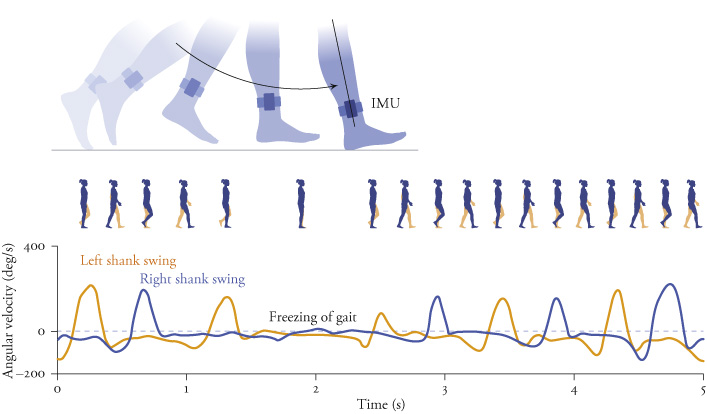
\includegraphics[width=1.0\linewidth]{chap7/7_4}
	\caption{惯性测量单元可以测量小腿在矢状面上的角速度(上图),从而检测帕金森病患者在生活环境中导航时出现的步态冻结(下图)\cite{o2020turning}。 \label{fig:7_4}}
\end{figure}


\begin{figure}[!htb]
	\centering
	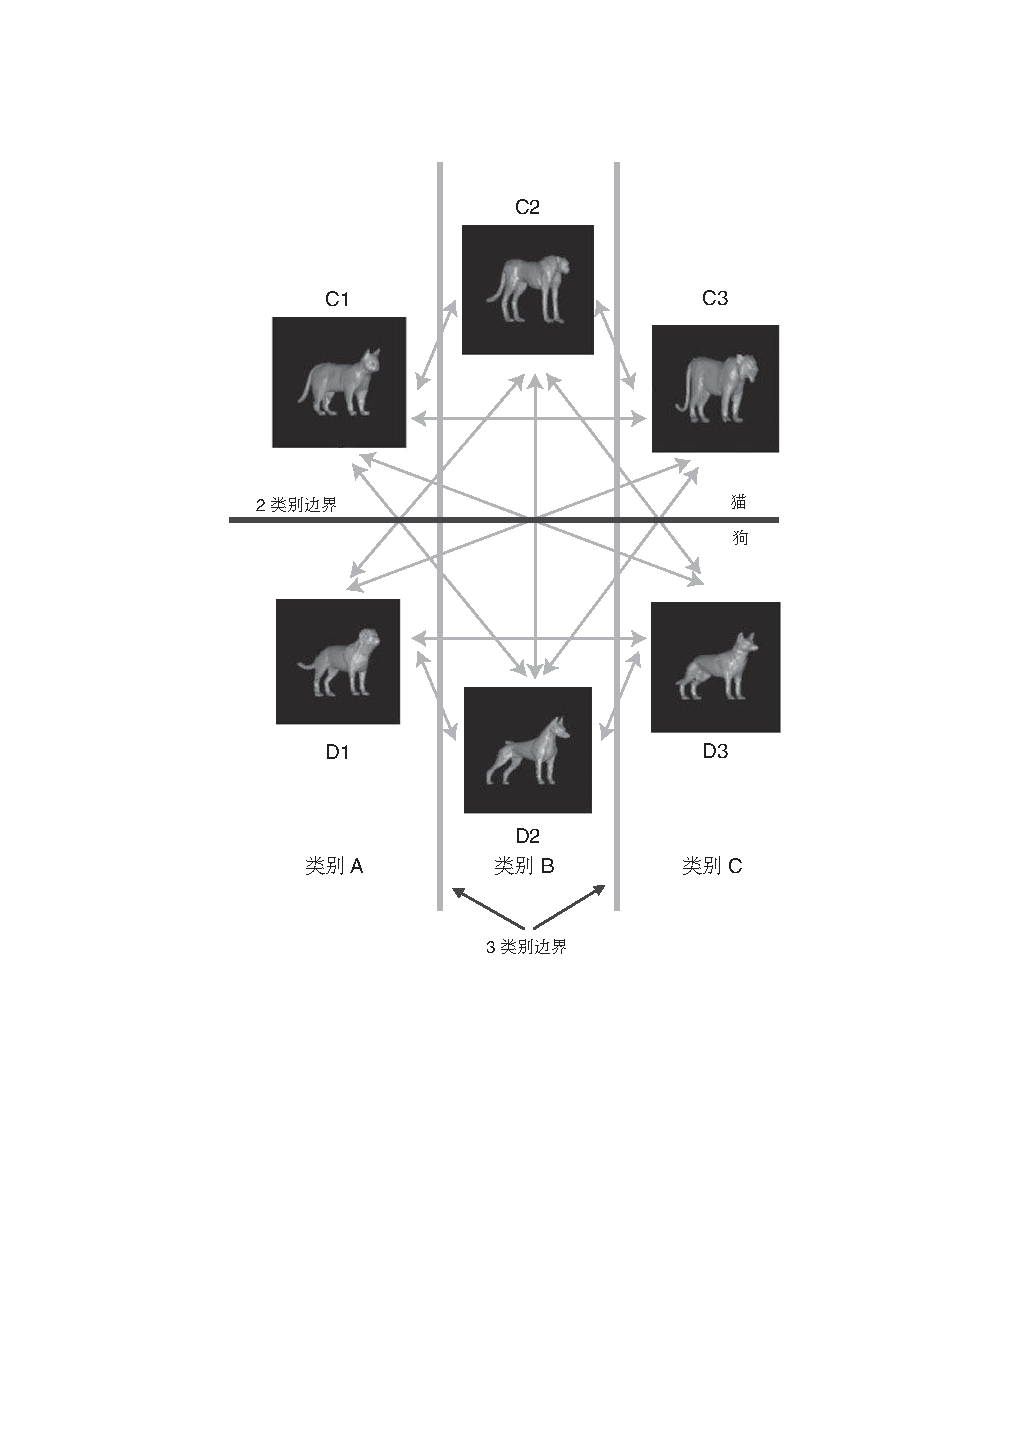
\includegraphics[width=1.0\linewidth]{chap7/7_5}
	\caption{用于监测运动员健康的运动学测量。
		配备惯性测量装置的护齿可测量颅骨运动。头部损伤标准 (HIC) 与总加速度曲线下的面积成正比。
		在本例中,15 毫秒时间窗口的安全阈值仅在 14.6 毫秒内累积,导致创伤性脑损伤\cite{hernandez2015six}。 \label{fig:7_5}}
\end{figure}



\section{光学动作捕捉}

动作捕捉(Motion Capture,简称“mocap”)已发展了近一个世纪。
除了在生物力学领域的作用外,它也是娱乐产业不可或缺的一部分。
为了制作电影和电子游戏中的角色动画,我们需要从现实场景(演员在房间里挥舞着棍子)到一系列图像(外星人用网捕捉蝴蝶)。
在生物力学领域,我们某种程度上逆转了这个过程:我们利用一系列图像来确定底层骨骼和肌肉是如何产生可观察到的运动的。


无论是在电影工作室还是生物力学实验室,技术都是一样的。我们将小型球形反射标记物固定在受试者的皮肤上或固定在板上,然后将其固定在受试者的身体上(图~\ref{fig:7_6})。
摄像机通常使用红外光来跟踪这些标记物的运动。
在红外光谱下工作有两个好处:它可以减少环境光的影响,并允许脉冲照明以减少运动模糊伪影。
如果我们使用可见光,频闪效果会非常令人分心。


\begin{figure}[!htb]
	\centering
	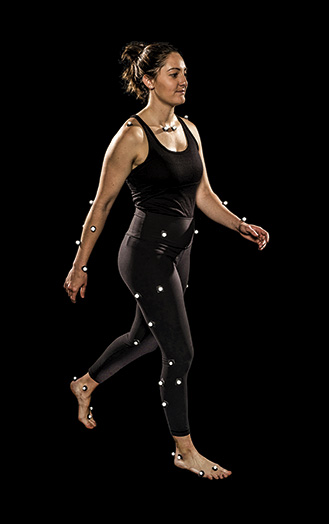
\includegraphics[width=0.5\linewidth]{chap7/7_6}
	\caption{光学运动捕捉 (mocap) 是一种流行的量化运动技术。
		我们可以通过皮肤上点的轨迹来估计底层骨骼的运动。 \label{fig:7_6}}
\end{figure}


一般来说,必须在一个身体部位上放置 3 个非共线标记,才能确定其在空间中的位置和方向。
如果假设某些标记与相邻部位共用(例如,假设膝盖外侧的标记相对于大腿和小腿保持固定),则少于 $3n$ 个标记即可追踪 $n$ 个身体部位。
也可以通过使用底层骨架的运动学模型来减少标记的数量。
然而,使用更多标记可能会改善某些逆运动学算法的关节角度估计。


每个摄像机记录一系列二维图像,捕捉每个标记在该摄像机局部二维图像平面中随时间变化的位置(图~\ref{fig:7_7})。
对于每个时间帧,计算机会将所有摄像机的位置信息与每个摄像机在空间中的相对位置和方向(在之前的校准过程中确定)相结合,以估计每个标记相对于“全局”实验室参考系的三维位置。
由于单幅图像无法提供摄像机与标记之间距离的精确信息,因此每个标记必须至少被两个摄像机可见才能确定其在空间中的位置。
增加实验室中摄像机的数量和它们之间的距离可以改进标记位置估计,解释受试者移动时发生的暂时性标记遮挡,并扩大可测量受试者运动的体积。
两到四个摄像机对于二维分析可能足够;大体积的三维分析可能需要数十个摄像机。
当动作捕捉系统校准并正确操作时,在典型的生物力学实验中,标记测量误差不会超过几毫米。


\begin{figure}[!htb]
	\centering
	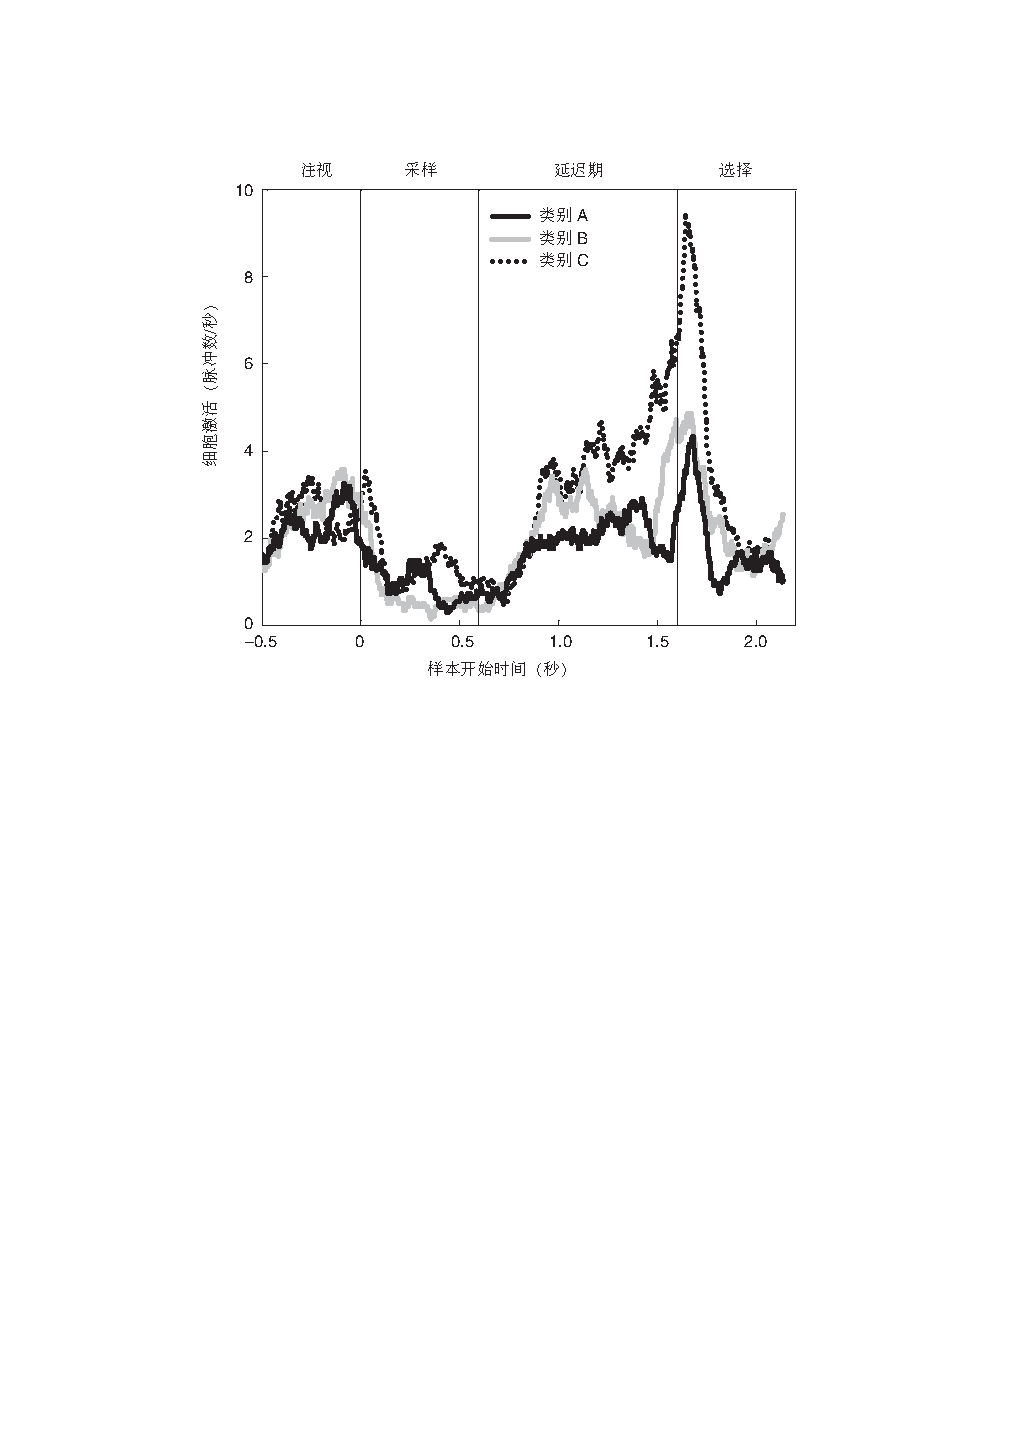
\includegraphics[width=1.0\linewidth]{chap7/7_7}
	\caption{每个标记点的位置在每个相机的局部二维图像平面中确定(例如,通过计算每个照明像素区域的质心,并按强度加权;参见插图中的十字准线)。
		然后,将这些二维位置与相机校准期间获得的信息相结合,计算出每个标记点在空间中相对于全局参考系的最佳位置估计值。  \label{fig:7_7}}
\end{figure}


实验测量误差的最大来源是软组织的运动。
当我们移动时,肌肉会膨胀,脂肪会晃动,皮肤会拉伸,从而改变安装在皮肤上的标记物与我们想要追踪的下层骨骼之间的关系。
软组织伪影不可避免,但可以通过将标记物放置在战略位置并使用考虑这些伪影的算法来减少其影响。
常用的标记物放置方案有几种;选择合适的方案在一定程度上取决于所进行研究的目标和所使用的逆运动学算法。
标记物通常放置在软组织运动相对较低的骨性解剖标志上,例如踝关节处的胫骨和腓骨踝。


在脂肪较多的位置或因为标记会干扰所研究的运动(例如,行走时放置在膝盖内侧)而将标记放置在解剖标志上可能不切实际。
在这种情况下,可以通过将解剖标志(例如,大转子)的位置与附近安装在皮肤上的标记的位置关联起来定义“虚拟标记”。
例如,在研究肥胖受试者时,我们将已知长度的校准棒压在皮肤上,直到棒的尖端到达解剖标志。
我们捕获单帧视频,以根据沿棒长度安装的标记的位置计算尖端的位置。
这些信息为我们提供了标记在皮肤上的位置和解剖标志的位置之间的关系,然后我们可以使用它来估计运动试验期间解剖标志的轨迹。
在关节中心定义虚拟标记也很有用,当关节在很大运动范围内移动时,可以使用安装在皮肤上的标记的轨迹来估计虚拟标记的位置。


即使创建了虚拟标记点,我们通常仍需要做更多工作才能使视频数据适合分析。
例如,我们通常希望通过对测量的位置数据求导来获取速度数据。
但微分会放大这些数据通常包含的高频噪声。
避免这种情况的一种方法是用低通滤波器平滑数据,从而消除高频运动。
但我们必须小心,避免滤除有意义的信息。由于感兴趣的频率范围取决于所研究的活动,因此合适的滤波器截止频率也取决于所研究的活动。
例如,我们可能对高达约 3 Hz 的频率感兴趣,用于研究姿势;
6 Hz 的频率感兴趣,用于研究行走;10-15 Hz 的频率感兴趣,用于研究跑步。
相比之下,高达 300 Hz 的频率可能与研究跑步时脚跟着地过程中运动的快速变化相关。
遗憾的是,软组织伪影通常出现在与目标信号相同的频率范围内,因此我们需要通过策略性标记点定位和专门设计用于考虑这些误差的算法来解决这些误差。


在分析原始视频数据之前,我们还会使用另外两种方法对其进行处理。
首先,在实验过程中,标记点通常会暂时被遮挡在摄像机视野之外,因此测量到的这些标记点的轨迹不完整。
可以使用插值法近似计算缺失的短片段;如果存在足够多的其他标记点,则可以通过忽略被遮挡的标记点来弥补较长的间隙。
其次,摄像机无法区分回射式光学标记点;必须在每一帧视频中为每个标记点添加标签。
我们可能需要手动分配这些标签,或者纠正自动标记方法造成的错误。
为了彻底避免标记点标记问题,可以使用发光的“主动”标记点代替上述回射式“被动”标记点。
主动标记点可以按顺序脉冲发光,以便每次只有一个标记点​​亮,从而实现唯一可识别。
尽管有此优势,但在我的实验室中,我们很少使用主动标记点。
许多系统需要电源和线缆,这可能会妨碍受试者的运动,而且每个标记点的脉冲频率(即数据采集速率)会随着标记点数量的增加而降低。
例如,一个以 1 kHz 频率运行的动捕系统,如果以 100 Hz 的频率脉冲,则只能准确捕捉 10 个标记点。
图~\ref{fig:7_8}~总结了从动捕数据计算关节角度的典型流程,并在下文进行描述。


\begin{figure}[!htb]
	\centering
	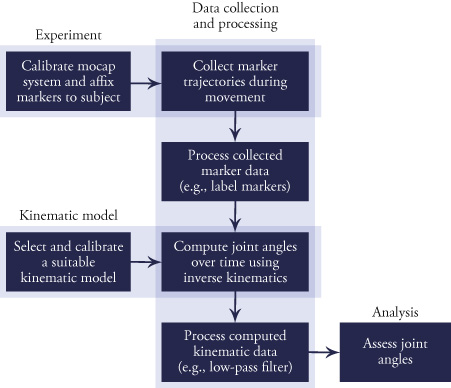
\includegraphics[width=0.75\linewidth]{chap7/7_8}
	\caption{从动作捕捉数据计算关节角度的典型流程。
		通过校准后的动作捕捉系统记录安装在皮肤上的标记点的运动轨迹。
		然后,利用受试者的运动学模型,根据 3D 标记点位置估计骨骼关节角度。 \label{fig:7_8}}
\end{figure}


从迈布里奇事件到现代,基于视频的分析一直是运动研究的主力。
未来,仅使用视频的无标记运动捕捉技术将更加精准,普及度也将进一步提升。
穿戴式加速度计和惯性测量单元 (IMU) 将显著扩展可开展的生物力学研究类型,并增加参与研究的人数。
然而,在本章的其余部分,我们将重点介绍目前在生物力学研究和临床运动捕捉实验室中最常用的技术,这些技术用于收集光学标记轨迹并计算骨骼关节运动学。


\section{无约束逆运动学}

一种常用的根据标记轨迹估算关节角度的方法是,首先根据附着在每个身体部位上的标记的位置,建立一个固定在该部位上的参考系(图~\ref{fig:7_9})。
然后,将固定在相邻部位上的参考系的相对方向解释为连接这些部位的关节角度(图~\ref{fig:7_10})。
我们将这种方法称为“无约束”逆运动学,因为它对肢体长度或隐含骨骼模型的关节运动没有任何约束或限制。 
(这种方法也被称为“直接法”,因为关节角度是根据标记位置“直接”计算出来的。
我们不鼓励使用这个术语,以免与“直接运动学”混淆,“直接运动学”是“正向运动学”的同义词,它描述了根据关节角度计算标记位置的相反过程。)
请注意,我们通常也对关节的角速度和角加速度感兴趣,但我们假设关节角度可以对时间进行微分(如有必要,在滤波之后)以获得这些量。


\begin{figure}[!htb]
	\centering
	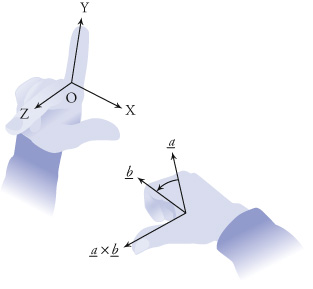
\includegraphics[width=0.55\linewidth]{chap7/7_9}
	\caption{固定在物体上的参考系由物体上的一点(参考系的“原点”,O)和三个正交轴(X、Y 和 Z)定义。
		按照惯例,我们使用“右手”参考系:
		如果伸出右手的拇指和食指,并使其与 X 和 Y 轴对齐,则中指指向远离手掌的方向时(左),将与 Z 轴对齐。
		如果将右手的手指从 $\underline{a}$ 弯曲到 $\underline{b}$ ,则完全伸展的拇指指向 $\underline{a} \times \underline{b}$ 的方向(右)。在右手坐标系中,$\hat{x} \times \hat{b} = \hat{z}$ 。 \label{fig:7_9}}
\end{figure}


\begin{figure}[!htb]
	\centering
	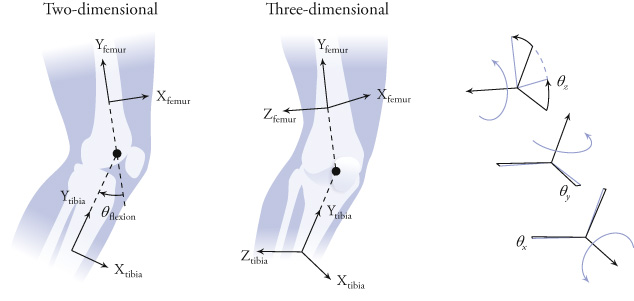
\includegraphics[width=1.0\linewidth]{chap7/7_10}
	\caption{通过比较固定在相邻身体部位的参考系的方向,可以计算出关节角度。
		膝关节屈曲可以通过二维分析中的检查来计算(左图),但在计算三维空间中两个参考系之间的相对方向时,更正式的方法更为有用(右图)。 \label{fig:7_10}}
\end{figure}


假设我们试图测量受试者在整个步态周期中的膝关节屈曲角度(具体来说,是股骨和胫骨绕膝关节轴的夹角)。
在最简单的情况下,我们会追踪两个参考系随时间的运动:一个固定在股骨上,一个固定在胫骨上,两者均与解剖膝关节轴对齐。
膝关节角度可以简单地定义为这些参考系在与膝关节轴正交的平面上的相对方向(图~\ref{fig:7_10})。
然而,更常见的情况是,我们会追踪固定在大腿和小腿上的标记点的位置,并且必须进行两项额外的计算。
首先,我们必须通过根据标记点位置构建与身体固定的参考系来计算大腿和小腿身体部位的位置和方向。
其次,由于放置在股骨内上髁上的标记物可能被遮挡,并可能干扰受试者的步态,因此膝关节解剖轴的位置和方向通常无法直接追踪,还必须根据固定在大腿和小腿上的标记物的位置来确定。
显然,这种情况更为复杂,本节的其余部分将详细描述无约束逆运动学方法的每个步骤。


标记的数量和位置可能因研究目标、被追踪的运动以及用于分析的软件而异。
通常使用两组标记,一组用于定义解剖参考框架,另一组用于定义追踪参考框架(图~\ref{fig:7_11})。
解剖参考框架代表底层骨骼结构,通过在解剖标志上放置标记来定义。
例如,固定在股骨上的解剖参考框架可以定义如下:


\begin{figure}[!htb]
	\centering
	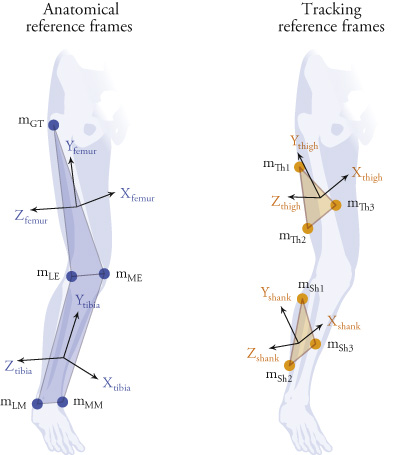
\includegraphics[width=0.75\linewidth]{chap7/7_11}
	\caption{通过安装在解剖标志上的标记(解剖参考框架)和安装在身体段上的标记(跟踪参考框架)确定的身体固定参考框架;m = 标记,GT = 大转子,ME/LE = 内/外股骨上髁,MM/LM = 内/外踝,Th = 大腿,Sh = 小腿。 \label{fig:7_11}}
\end{figure}


\begin{itemize}
	\item 原点位于大转子标记($m_{GT}$)与膝关节中心(股骨内上髁标记$m_{ME}$、股骨外上髁标记$m_{LE}$的中点)的中点;
	\item $Z_\text{femur}$ 平行于膝关节轴,其定义为从内侧到外侧股骨上髁标记的矢量,标准化为单位长度;
	\item $X_{femur}$ 是 $Z_{femur}$ 与从大转子标记到股骨上髁标记之一的矢量的叉积,标准化为单位长度;
	\item $Y_{femur}$ 是 $Z_{femur}$ 和 $X_{femur}$ 的叉积,它完成了右手参考系(图~\ref{fig:7_9})。
\end{itemize}


类似地,我们也可以定义一个固定在胫骨上的参考系,同样使用股骨上髁标记来定义Z轴。
然后,我们可以将膝关节屈曲角度定义为胫骨参考系相对于股骨参考系绕(平行)Z轴的夹角。


追踪参考系也固定在身体各节段上,但它们可能与解剖学相关的轴不对齐。
追踪参考系由每个节段上至少三个非共线标记点定义。
这些标记点不必与用于定义解剖参考系的标记点不同,但它们应放置在整个实验过程中始终可见且软组织运动相对较小的位置。
例如,可以使用大转子和股骨外上髁标记点以及放置在大腿某处的另一个标记点​​来定义大腿参考系。
然后,可以根据这些标记点定义一个正交的右手参考系。
追踪参考系很有用,因为它们使我们能够将标记点放置在比解剖学标志更方便的位置。
我们仍然需要解剖学参考系来计算关节角度,但一旦知道追踪参考系,就可以轻松计算解剖参考系,如下一节所述。



\section{变换矩阵}

在上面的例子中,计算膝关节屈曲角度非常简单,因为固定在股骨和胫骨上的解剖参考系是用平行的Z轴定义的。
因此,一个参考系相对于另一个参考系的方向可以用绕公共Z轴的单个旋转角度来描述。
通常,我们用三个角度(而不是一个)来关联两个任意方向的参考系,这些角度被称为欧拉角(以18世纪数学家莱昂哈德$\cdot$欧拉的名字命名)。
这些角度总是描述绕三个轴的一系列连续旋转,但旋转的顺序并不唯一。
例如,你可以描述绕X轴旋转,然后绕Y轴旋转,最后绕Z轴旋转。
或者,你可以先绕Z轴旋转,或者绕旋转后的Y轴旋转,而不是绕原始轴旋转。
这三个轴的选择有一些比其他轴更常见。
例如,在航空学中,传统上选择旋转轴的三个角度分别是偏航角、俯仰角和滚转角(图~\ref{fig:7_12})。
这组旋转序列被称为Z-Y-X体固旋转序列,之所以称之为“体固”是因为每次旋转都围绕着附着在体上的框架进行。
(另一种旋转序列被称为“空间固”序列,因为每次旋转都围绕着实验室框架的某个轴进行。)


\begin{figure}[!htb]
	\centering
	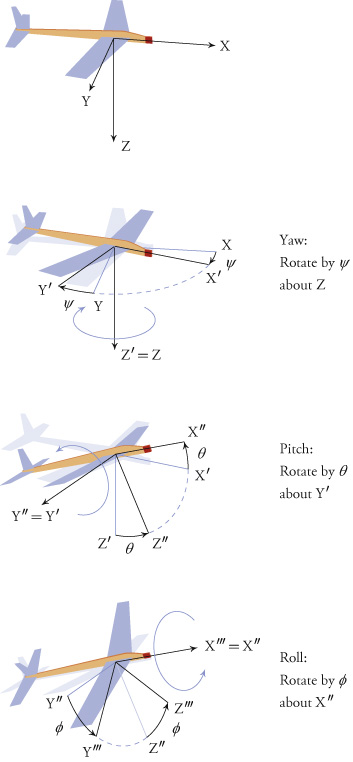
\includegraphics[width=0.5\linewidth]{chap7/7_12}
	\caption{Y aw、pitch 和 roll 描述了流行的 Z–Y–X 机身固定旋转序列中的三个旋转角度。 \label{fig:7_12}}
\end{figure}


假设给定两个参考系 A 和 B,以及一个相对于参考系 B 坐标表示的点,我们希望计算该点相对于参考系 A 坐标的坐标。
我们可以通过旋转矩阵关联这两个参考系的方向,该矩阵是一个 $3\times3$ 矩阵 $^AR_B$,其列只是沿参考系 B 的 X、Y 和 Z 轴指向的单位向量的坐标,这些向量相对于参考系 A 坐标表示。
一旦我们知道了这个矩阵,我们就可以通过用矩阵 $^AR_B$ 乘以向量 $p_B$,将任意点 $p_B$ 在参考系 B 中的坐标转换为相应的在参考系 A 中的坐标:
%
\begin{equation}
	p_A = ^A R_B p_B
	\label{eq:7_1}
\end{equation}
%
类似地,我们可以通过将矩阵 $^BR_A$ 乘以向量 $p_A$,将任意点 $p_A$ 在 A 坐标系中的坐标转换为相应的 B 坐标系中的坐标。
同样,我们可以通过将公式~\ref{eq:7_1}~的每一边预乘以 $(^AR_B)^{−1}$,根据 $p_A$ 计算出 pB:
%
\begin{equation}
	( ^A R_B ) ^{-1} p_A = p_B
	\label{eq:7_2}
\end{equation}
%
这表明了以下关系:
%
\begin{equation}
	^R_A = ( ^A R_B ) ^{-1}
	\label{eq_7_3}
\end{equation}

事实上,旋转矩阵满足一种称为正交性的性质,这意味着旋转矩阵的逆等于它的转置:
%
\begin{equation}
	( ^A R_B )^{-1} = ( ^A R_B )^T
	\label{eq:7_4}
\end{equation}

因此,我们也可以将 $^AR_B$ 定义为旋转矩阵,其行是沿框架 A 的 X、Y 和 Z 轴指向的单位向量的坐标,相对于框架 B 表示。


为了推导矩阵 $^AR_B$ 与一组特定的欧拉角之间的关系,我们将从一个类比开始。
想象一下,你正坐在一架准备起飞的飞机上,并定义了一个坐标系,其 X 轴指向机头,Y 轴指向右翼,Z 轴指向下方(图~\ref{fig:7_12})。
我们将此坐标系称为实验室坐标系。
现在,系好安全带,想象飞机执行三个机动动作。
首先,它在滑行至跑道时向右转弯,绕 Z 轴旋转一个角度 $\psi$。
(目前,我们将忽略飞机沿滑行道向下移动的距离,仅考虑其方向的变化。)
这种机动动作在航空学中称为“偏航”,它会为 X′、Y′ 和 Z′ 轴产生一组新的基向量。
注意,Z′ = Z,因为“向下”向量的方向并没有因右转而改变。
轴 {X′, Y′, Z′} 定义了一个新的参考系,我们将其称为参考系 1 或 f1。


其次,飞机起飞,机头抬升(绕 Y′ 轴旋转)一个角度 $\theta$。
飞行员称之为“俯仰”的这个运动,会产生另一个新的参考系 f2 = {X″, Y″, Z″},如图~\ref{fig:7_12}~所示。
这次 Y″ = Y′,因为机头向上俯仰不会影响右机翼的指向。


第三,飞机向一侧倾斜,右机翼向下倾斜(绕 X″ 轴旋转)一个角度 $\phi$。
这种动作在航空学中称为“滚转”,由此产生的第三个参考系我们称之为机身参考系:机身 = {X′′′, Y′′′, Z′′′}。
在这种情况下,X′′′ = X″,因为机翼向上或向下倾斜不会改变机头指向的方向。
通过这种方式,我们可以从惯性系或实验室固定参考系出发,按顺序执行上述三个动作,从而得到固定在空间中任何机身上的参考系。


我们如何将(可移动的)固定身体参考系转换回(静止的)固定实验室参考系?用符号表示,矩阵 $^{\text{lab}}R_{\text{body}}$ 是什么?
或者用文字表达,我们如何将来自固定身体传感器的测量值转换为我们偏好的实验室坐标系中的观测值?


借助飞机的类比,我们希望答案相对显而易见:我们撤销上述旋转序列。
为了从身体坐标系转换到实验室坐标系,我们首先从身体坐标系转换到 f2 坐标系。
然后,我们从 f2 坐标系转换到 f1 坐标系。
最后,我们从 f1 坐标系转换到实验室坐标系。
因此,我们计算旋转矩阵 $^\text{lab}R_\text{body}$ 如下:
%
\begin{equation}
	^\text{lab}R_\text{body} = 
		^\text{lab} R _\text{f1}
		^\text{f1} R _\text{f2}
		^\text{f2} R _\text{body}
	\label{eq:7_5}
\end{equation}


注意变换的顺序,一开始可能不太明显。
因为这些变换可以被认为是一系列函数,所以我们从右到左写出它们的复合函数,因此首先应用的是变换 $^\text{f2}R_\text{body}$(从身体坐标系到 f2 坐标系)。


上述分解的一大好处是,3 个旋转矩阵都具有非常简单的形式。
我们从 f1 坐标系到 lab 坐标系的变换开始:
% 参考:https://zhuanlan.zhihu.com/p/266267223
\begin{equation}
	^\text{lab} R_\text{f1} = 
		\begin{bmatrix} % 方括号为pmatrix
			cos \psi & -sin \psi & 0 \\
			sin \psi & cos \psi  & 0 \\
			0 & 0 & 1
		\end{bmatrix}
	\label{eq:7_6}
\end{equation}


要理解矩阵为何呈现这种形式,请记住旋转矩阵的第一列表示新的 X′ 轴相对于原始 {X, Y, Z} 参考系的坐标。
并且记住 X′ 是什么:飞机机头绕 Z 轴旋转 ψ 角后指向的方向。
该方向的单位向量为 $(cos \psi, sin \psi, 0)$,它们正是矩阵第一列的元素。类似地,第三列表示 {X, Y, Z} 参考系中 Z′ 轴的方向。
记住 Z′ = Z,正如我们之前指出的,我们得出结论,该方向的单位向量就是 (0, 0, 1),因此它就是旋转矩阵的第三列。


我们也可以通过将 f1 框架中各坐标轴上的点变换到 Lab 框架来检查这个矩阵。
例如,一只坐在右翼的鸟,在 Lab 框架中可能具有以下坐标:
%
\begin{equation}
	p_\text{lab}
	= ^\text{lab} R_\text{f1} p_\text{f1}
	= \begin{bmatrix}
		cos \psi & -sin \psi & 0 \\
		sin \psi & cos \psi & 0 \\
		0 & 0 & 1
	  \end{bmatrix}
	  %
	  \begin{bmatrix}
	  	0 \\
	  	1 \\
	  	0
	  \end{bmatrix}
	= \begin{bmatrix}
		-sin \psi \\
		cos \psi \\
		0
	\end{bmatrix}
	\label{eq:7_7}
\end{equation}


如果飞机右转($\sigma$ = 90 度),那么鸟儿最终会落在原来方向舵的位置。
鸟儿相对于原始参考系的坐标为 (-1, 0, 0)。
类似地,我们可以证明
%
\begin{equation}
	^\text{f1} R_\text{f2} = 
		\begin{bmatrix}
			cos \theta & 0 & sin \theta \\
			0 & 1 & 0 \\
			-sin \theta & 0 & cos \theta
		\end{bmatrix}
	\label{eq:7_8}
\end{equation}
并且
\begin{equation}
	^\text{f2} R_\text{body}
		= \begin{bmatrix}
			1 & 0 & 0 \\
			0 & cos \phi & -sin \phi \\
			0 & sin \psi & cos \phi
		\end{bmatrix}
	\label{eq:7_9}
\end{equation}


方程~\ref{eq:7_6}、\ref{eq:7_8}~和~\ref{eq:7_9}~中的矩阵被称为初等旋转矩阵,因为在每种情况下,固定于物体的坐标轴之一保持静止。
完整的旋转变换 $^{lab}R_\text{body}$ 由这 3 个初等旋转矩阵按规定顺序的乘积给出:
%
\begin{equation}
	\begin{aligned}
		^\text{lab} R_\text{body} & = 
			^\text{lab} R_\text{f1}
			^\text{f1} R_\text{f2}
			^\text{f2} R_\text{body} \\
		& = \begin{bmatrix}
			cos \theta cos \psi & 
			sin \phi sin \theta cos \psi - cos \phi sin \psi &
			cos \phi sin \theta cos \psi + sin \phi sin \psi \\
			% 
			cos \theta sin \psi &
			sin \phi sin \theta sin \psi + cos \phi cos \psi &
			cos \phi sin \theta sin \psi - sin \phi cos \psi \\
			%
			- sin \theta &  sin \phi cos \theta &  \cos \phi cos \theta
		\end{bmatrix} \\
		%
		& = \begin{bmatrix}
			r_{11}  & r_{12}  & r_{13} \\
			r_{21}  & r_{22}  & r_{23} \\
			r_{31}  & r_{32}  & r_{33}
		\end{bmatrix}
	\end{aligned}
	\label{eq:7_10}
\end{equation}
%
其中,每个元素 $r_{ij}$ 都是介于 0 和 1 之间的数字。
我们可以通过将任意旋转矩阵的元素设置为公式~\ref{eq:7_10}~中相应的三角表达式,从而根据该旋转矩阵的数值元素计算出角度 $\psi$、$\theta$ 和 $\phi$。
只有对三个角度施加限制,才能获得唯一解;一种策略是使用四象限(2 个参数)反正切函数 (atan2),如下所示:
%
\begin{equation}
	\begin{aligned}
		\phi & = atan2(r_{32}, r_{33}) \\
		\theta & = atan2(-r_{31}, \sqrt{r_{11}^2} + r_{21}^2) \\
		\psi & = atan2(r_{21}, r_{11})
	\end{aligned}
	\label{eq:7_11}
\end{equation}


注意,我们可以通过将数值项 $r_{ij}$ 与不同的符号旋转矩阵关联起来,计算出不同旋转序列(例如,先绕 X 轴旋转,再绕 Y′ 轴旋转,最后绕 Z″ 轴旋转)对应的角度。
我们只需计算公式~\ref{eq:7_10}~中一组不同的基本旋转矩阵的乘积即可。


在前面的讨论中,我们假设所有参考系都共享一个原点,因此仅通过旋转变换即可关联。
然而,附着在不同身体部位(例如大腿和小腿)的参考系通常具有不同的原点,因此它们不仅通过旋转关联,还通过平移关联。
通常,从参考系 B 中的坐标到参考系 A 中的坐标的变换是通过旋转 $^AR_B$ 和平移的组合来完成的:
%
\begin{equation}
	p_A = ^A R_B p_B + p_A^{A_0 B_0}
	\label{eq:7_12}
\end{equation}
%
其中 $p_A ^{A_o B_o}$ 是从 A 坐标系的原点 ($A_o$) 到 B 坐标系的原点 ($B_o$) 的位置向量,以 A 坐标系表示。
(注意,当 A 坐标系和 B 坐标系的原点重合时,公式~\ref{eq:7_12}~简化为公式~\ref{eq:7_1}。)
这种变换将旋转和平移结合在一起,可以方便地用一个 $4 \times 4$ 变换矩阵来表示,该矩阵可以捕捉 2 个坐标系之间的相对位置和方向:
% 5x5
\begin{equation}
	^A T_B = 
	\begin{bmatrix}
		& & & | & \\
		& ^A R_B & & | & p_A ^{A_0 B_0} \\
		& & & | & \\
		--& -- & -- & | & -- \\
		0 & 0 & 0 & | & 1
	\end{bmatrix}
	\label{eq:5_13}
\end{equation}


因此,在框架 B 中表达的点可以使用变换矩阵在框架 A 中表示如下:
%
\begin{equation}
	\begin{bmatrix}
		p_A \\
		1
	\end{bmatrix}
	=
	^A T_B
	\begin{bmatrix}
		p_B \\
		1
	\end{bmatrix}
	\label{eq:7_14}
\end{equation}

公式~\ref{eq:7_14}~有效地在公式~\ref{eq:7_12}~的右侧包含了偏移向量,同时保留了使用单个矩阵 ($^AT_B$) 关联两个帧的符号便利性。



最后,对于那些对数学特别感兴趣的读者,我们需要指出,用旋转矩阵(例如公式~\ref{eq:7_10})表示旋转并非总是最佳选择。
这种方法存在一个称为“万向节锁”的缺陷:当两个或多个旋转轴对齐时,无法表示某些旋转。
例如,如果图 7.12 中的俯仰 $\theta = −90$ 度,则 Z = X″,改变角度 $\psi$ 和 $\phi$ 对飞机的影响相同。
在坐标系运动范围有限的应用中,可以避免万向节锁。
但是,例如,如果你正在编写一个飞行模拟器,并且你希望用户能够流畅地翻筋斗,那么变换矩阵可能不是一个好的选择。
另一种表示方法称为四元数,可以避免万向节锁,但代价是使用更深奥的数学。


\section{利用无约束逆运动学计算关节角度}

变换矩阵的一大优势在于它简化了多个坐标系之间的导航。
具体来说,它使我们能够根据实验室框架中收集的数据,轻松计算出解剖关节角度。
回想一下,动捕系统记录的是安装在皮肤上的标记点相对于实验室中固定的参考框架的位置(图~\ref{fig:7_13})。
例如,为了计算膝关节屈曲角度,我们可以确定与固定在股骨和胫骨上的参考框架相关的变换矩阵:

\begin{figure}[!htb]
	\centering
	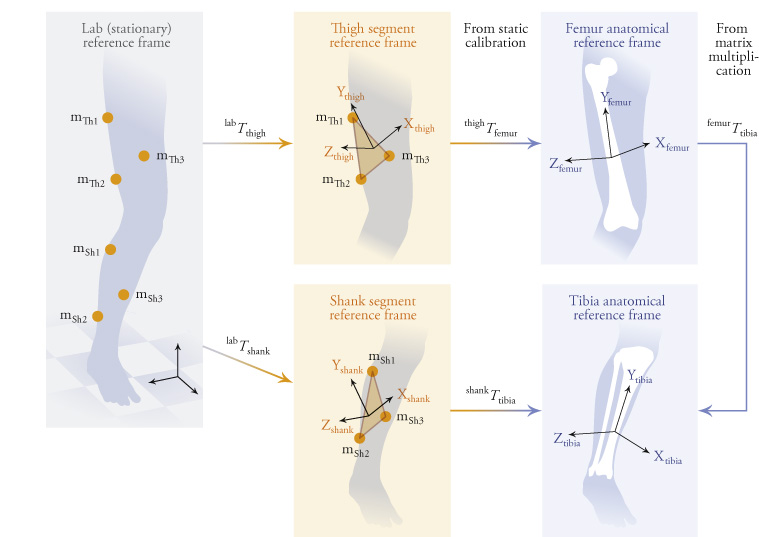
\includegraphics[width=1.0\linewidth]{chap7/7_13}
	\caption{任意两个参考系的相对位置和方向可以用 4$\times$4 变换矩阵 T 来描述,这有助于根据相对于全局参考系测量的标记位置来计算关节角度。 \label{fig:7_13}}
\end{figure}

\begin{equation}
	^\text{femur} T_\text{tibia} = 
		^\text{femur} T_\text{thigh}
		^\text{thigh} T_\text{lab}
		^\text{lab} T_\text{shank}
		^\text{shank} T_\text{tibia}
	\label{eq:7_15}
\end{equation}


从右到左阅读此公式描述了胫骨框架中的坐标与股骨框架中的坐标之间的关系。


假设没有骨骼变形也没有软组织运动,大腿和小腿跟踪参考框架可以通过恒定变换分别与股骨和胫骨解剖框架相关联。
这些变换矩阵($^\text{thigh}T_{femur}$ 和 $^\text{shank}T_\text{tibia}$)可以通过在“静态校准试验”期间关联跟踪和解剖参考框架来获得,其中两组标记都连接到受试者并在站立期间收集数据。
变换 $^\text{lab}T_\text{thigh}$ 和 $^\text{lab}T_\text{shank}$ 是通过根据运动试验每个时刻由动作捕捉系统记录的标记位置计算大腿和小腿参考框架获得的。
然后可以使用公式~\ref{eq:7_10}~从 $^\text{femur}T_\text{tibia}$ 变换矩阵中提取膝关节屈曲角度。
如果股骨和胫骨框架具有平行的 Z 轴,则可以使用更简单的公式~\ref{eq:7_6},如图~\ref{fig:7_11}~所示。


无约束逆运动学方法因其易于实现且在许多商业软件包中可用而广受欢迎。
然而,这种方法有一个主要局限性:它没有考虑解剖学施加的约束。
因此,模型的身体节段可能会改变长度,其关节可能会在运动过程中脱位,并且算法对软组织运动敏感。
无约束逆运动学模型会产生误差,影响计算出的关节角度以及所有后续计算(例如关节力矩和肌肉力)。
我更倾向于使用另一种方法,下文将对此进行介绍。



\text{约束逆运动学}

约束逆运动学方法利用优化方法,最小化固定在受试者身上的实验标记点位置与固定在受试者骨骼运动模型上的相应标记点位置之间的距离(图~\ref{fig:7_14})。
该模型由刚体构成,这些刚体通过解剖学上精确的关节相互连接,这些关节只允许进行可靠测量的运动。
模型会进行缩放以匹配受试者的尺寸。
与无约束逆运动学方法相比,使用结合了受试者几何形状和活动性知识的模型可以更精确地估计关节角度。
此类模型中的约束将可能的解集限制为那些代表解剖学上可行运动的解。
例如,骨骼的长度不能随时间变化,关节也不能脱位或超出定义的解剖极限。
以下目标函数在每个时间点上针对模型的广义坐标(例如,其在空间中的位置和每个关节的角度)进行最小化:


\begin{figure}[!htb]
	\centering
	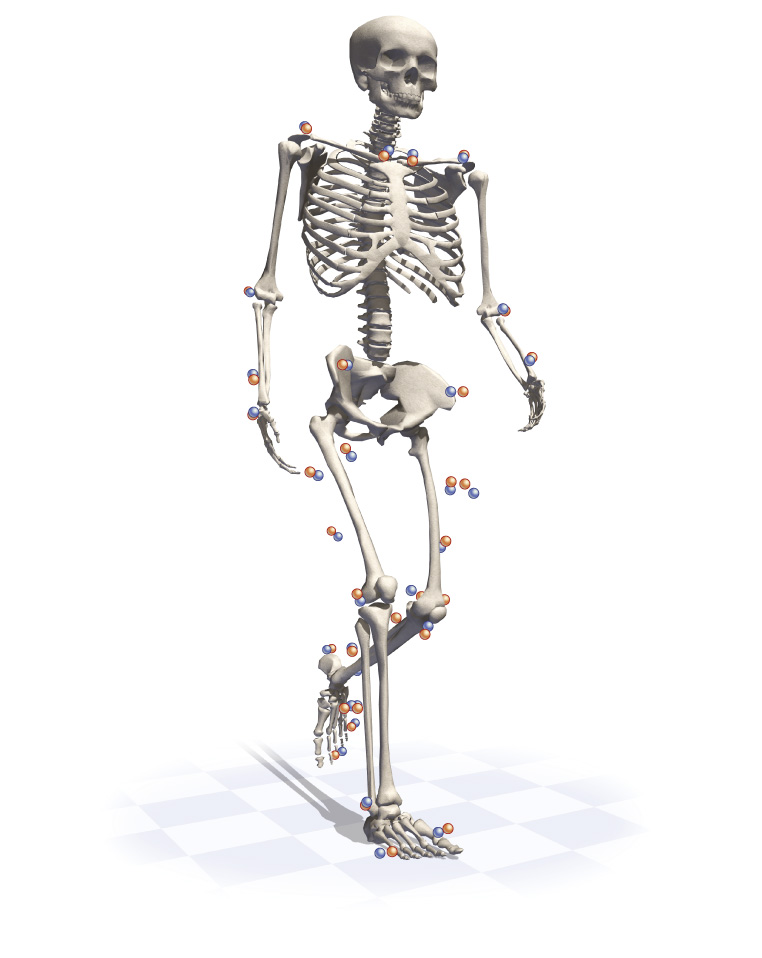
\includegraphics[width=0.9\linewidth]{chap7/7_14}
	\caption{如果解决方案受到底层骨架模型的约束,则逆运动学算法可以产生更准确的关节角度估计,其中放置在模型上的标记(橙色)跟踪放置在主体上的标记的轨迹(蓝色)。 \label{fig:7_14}}
\end{figure}


\begin{equation}
	J(\underline{q}) = 
		\sum_{k \in \text{Markders}} 
		w_k
		\Vert \underline{k}^\text{exp} - \underline{k}_k (\underline{q}) \Vert
	\label{eq:7_16}
\end{equation}













